\subsection{Anisotropic disorder}
\label{sec:flat-anisotropic}

For $a=1$, we distinguish edge, screw and $45^\circ$ mean orientations.
Their angles are $\beta=90^\circ$, $0^\circ$ and $45^\circ$,
respectively, measured between $\hat{\boldsymbol b}$ and the $x$ axis.

\subsubsection{Edge}
\label{sec:flat-edge}

For the edge orientation, $\hat{\boldsymbol b}$ is perpendicular to the
mean interface direction. We use the same system sizes, aspect ratio
and numbers of realizations as in the isotropic case, and add $32$
realizations at $L_x=4096$.
Figure~\ref{fig:edge-profiles} shows the contour and the two height
representations for one depinning configuration.

\begin{figure}[H]
 \centering
 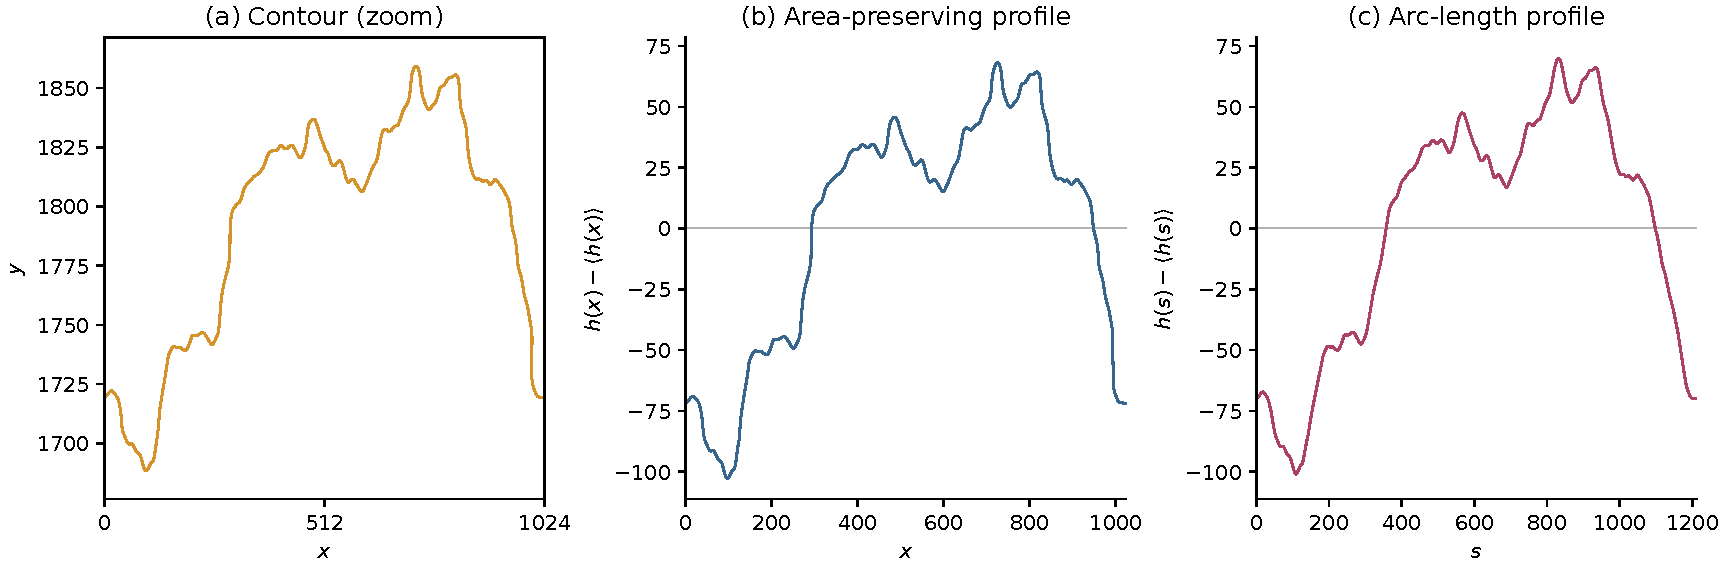
\includegraphics[width=\linewidth]{fig3_edge_profiles.pdf}
 \caption{Flat edge interface with anisotropic disorder ($a=1$) at
 $L_x=1024$, with perimeter $P=1212.86$.
 (a) Enlarged view of the full depinning contour.
 (b) Area-preserving profile $h(x)$.
 (c) Height $h(s)=y(s)$ along the contour, parametrized by arc length
 $s\in[0,P)$.
 In (b,c), the means $\langle h(x)\rangle$ and
 $\langle h(s)\rangle$ are subtracted, respectively.}
 \label{fig:edge-profiles}
\end{figure}

The mean perimeter grows approximately as
$\mathbb E[P]\propto L_x^{1.005}$, as shown in
Fig.~\ref{fig:edge-scaling}(a).
The ratio $\mathbb E[P]/L_x$ remains close to $1.12$ at the largest sizes.
Figure~\ref{fig:edge-scaling}(b) shows $S(n)$, with lines of slope
$-2.26$ (qKPZ, $\zeta=0.63$) and $-3.5$ ($\zeta=1.25$).
The lowest modes, $2\leq n\leq8$, give $\zeta\simeq0.64$, $0.64$ and
$0.67$ for $h_x$, and $0.68$ for $h_s$, at $L_x=1024$, $2048$ and $4096$.
These values are close to qKPZ and do not drift with $L_x$.
At $L_x=4096$ the first quarter of the modes, $2\leq n\leq22$, gives
$\zeta\simeq0.68$ for $h_x$ and $0.71$ for $h_s$.
At larger $n$ the spectra are steeper, with $\zeta\simeq0.94$ and
$1.04$.
For $q\leq0.03$, the binned spectra give $\zeta_x\simeq0.59$, $0.63$ and
$0.69$, and $\zeta_s\simeq0.57$, $0.64$ and $0.73$, at the same sizes.
At $L_x=4096$, $q\leq0.015$ gives $\zeta_x\simeq0.65$ and
$\zeta_s\simeq0.62$.
The increase at $q\leq0.03$ therefore comes from the start of the
crossover to steeper spectra near $q\simeq0.03$.
The mean depinning force decreases with $L_x$.
A fit $\mathbb E[F_d]=F_c+AL_x^{-1/\nu}$ for $256\leq L_x\leq4096$
gives $1/\nu=0.56\pm0.08$, consistent with the qKPZ value $0.58$
($\nu=1.733$) and below the qEW value $0.75$ ($\nu=4/3$).

\begin{figure}[H]
 \centering
 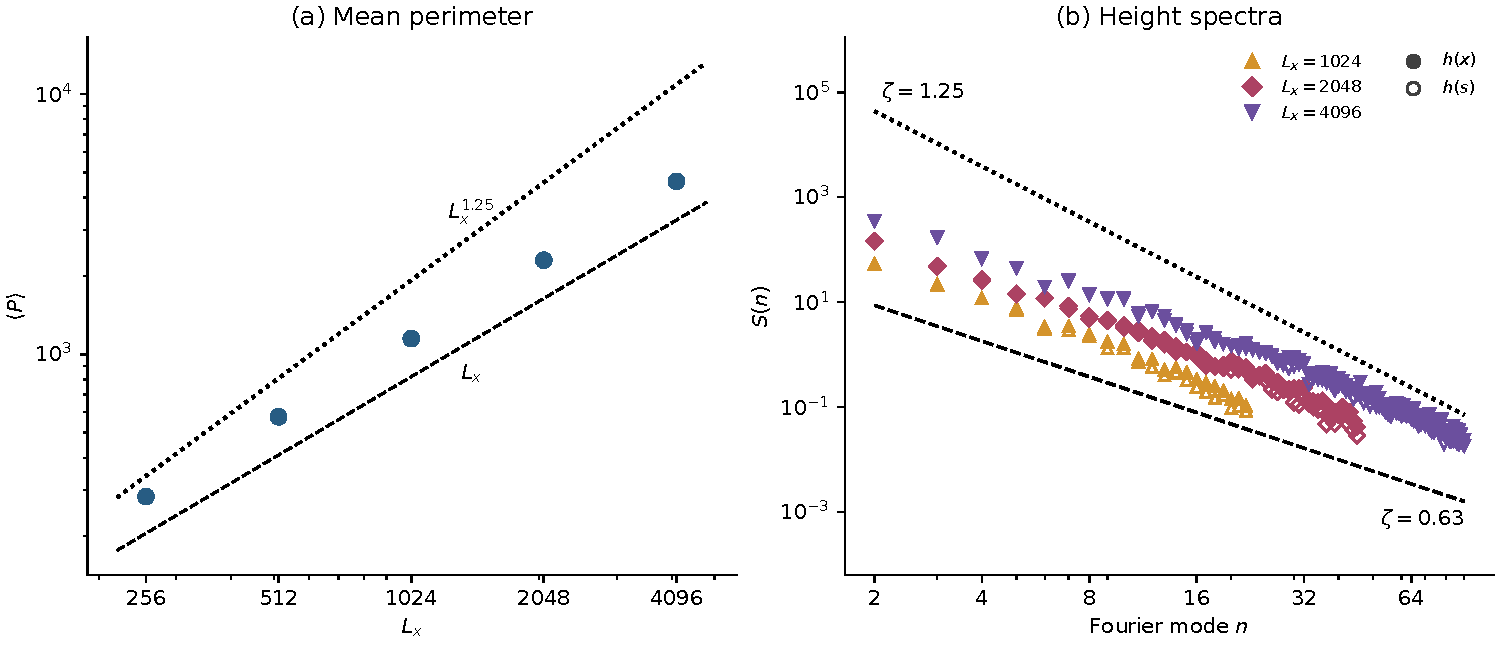
\includegraphics[width=\linewidth]{fig4_edge_scaling.pdf}
 \caption{Flat edge interfaces with anisotropic disorder ($a=1$),
 $\hat{\boldsymbol b}$ perpendicular to the mean interface direction,
 and $L_y=2L_x$.
 (a) Mean perimeter versus $L_x$.
 Error bars give $95\%$ bootstrap intervals for the mean.
 The black dashed and dotted lines have slopes $1$ and $1.25$,
 respectively.
 (b) Spectra $S(n)=\langle|\widehat h_n|^2\rangle$ versus the mode
 index $n$ for $L_x=1024$, $2048$ and $4096$, with
 $2\leq n\leq45L_x/2048$.
 Filled symbols represent $h_x(x)$ and open symbols represent $h_s(s)$.
 The black dashed and dotted lines have slopes $-2.26$ ($\zeta=0.63$)
 and $-3.5$ ($\zeta=1.25$), with freely chosen amplitudes.
 Each contour has equal weight in the disorder average.}
 \label{fig:edge-scaling}
\end{figure}


\subsubsection{Screw}
\label{sec:flat-screw}

For the screw orientation, $\hat{\boldsymbol b}$ is parallel to the
mean interface direction. We use the same system sizes, aspect ratio
and numbers of realizations as above.
Figure~\ref{fig:screw-profiles} shows a depinning configuration with
long, nearly straight segments.

\begin{figure}[H]
 \centering
 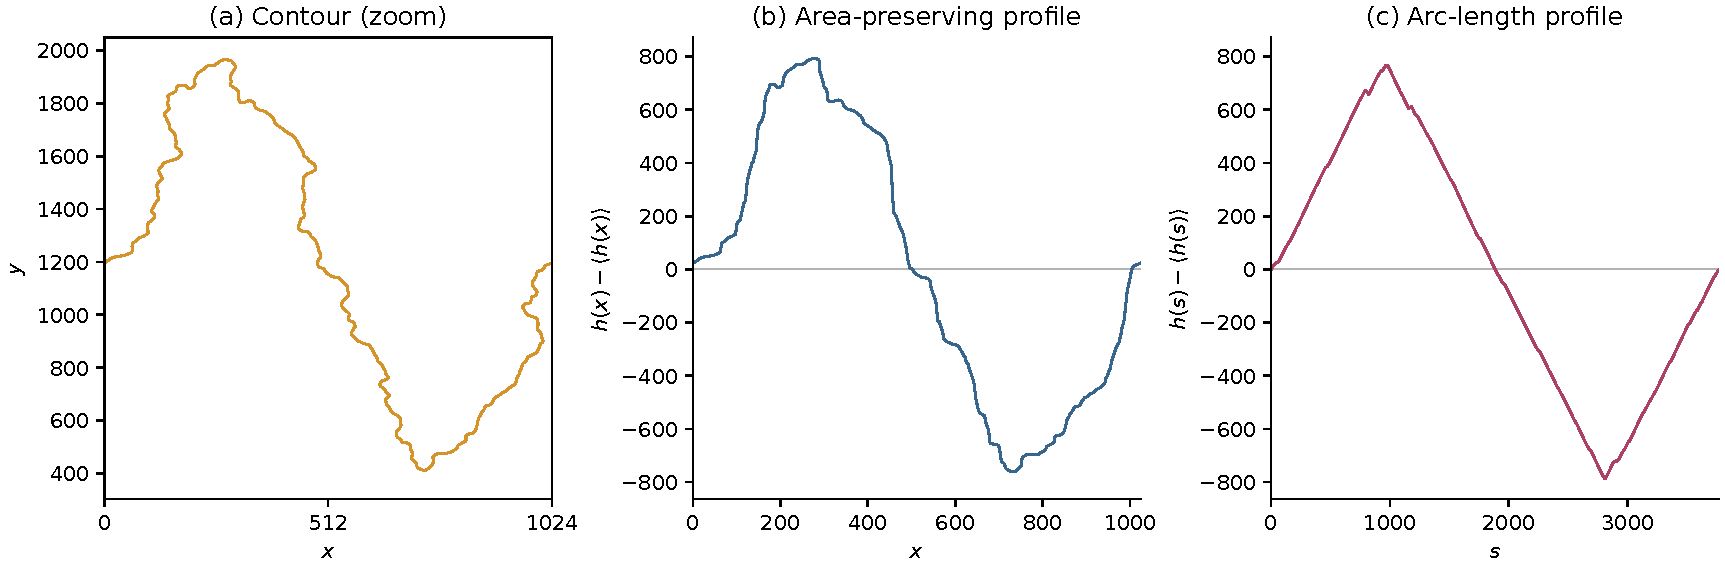
\includegraphics[width=\linewidth]{fig5_screw_profiles.pdf}
 \caption{Flat screw interface with anisotropic disorder ($a=1$) at
 $L_x=1024$, with perimeter $P=3766.36$.
 (a) Enlarged view of the full depinning contour.
 (b) Area-preserving profile $h(x)$.
 (c) Height $h(s)=y(s)$ along the contour, parametrized by arc length
 $s\in[0,P)$.
 In (b,c), the means $\langle h(x)\rangle$ and
 $\langle h(s)\rangle$ are subtracted, respectively.}
 \label{fig:screw-profiles}
\end{figure}

The mean perimeter grows approximately as
$\mathbb E[P]\propto L_x^{1.45}$, as shown in
Fig.~\ref{fig:screw-scaling}(a).
The ratio $\mathbb E[P]/L_x$ increases from $1.92$ at $L_x=256$
to $4.81$ at $L_x=2048$.
Figure~\ref{fig:screw-scaling}(b) shows $S(n)$, with lines of slope
$-3.9$ ($\zeta=1.45$) and $-3.5$ ($\zeta=1.25$).
Over all the modes shown, $h_s$ gives $\zeta\simeq1.46$ and $h_x$
gives $\zeta\simeq1.06$ at $L_x=2048$.
At $L_x=2048$ and $q\leq0.03$, the effective exponents are
$\zeta_x\simeq1.24$ and $\zeta_s\simeq1.37$.
These slopes depend on the fitted range and do not establish a
universality class for this faceted regime.

\begin{figure}[H]
 \centering
 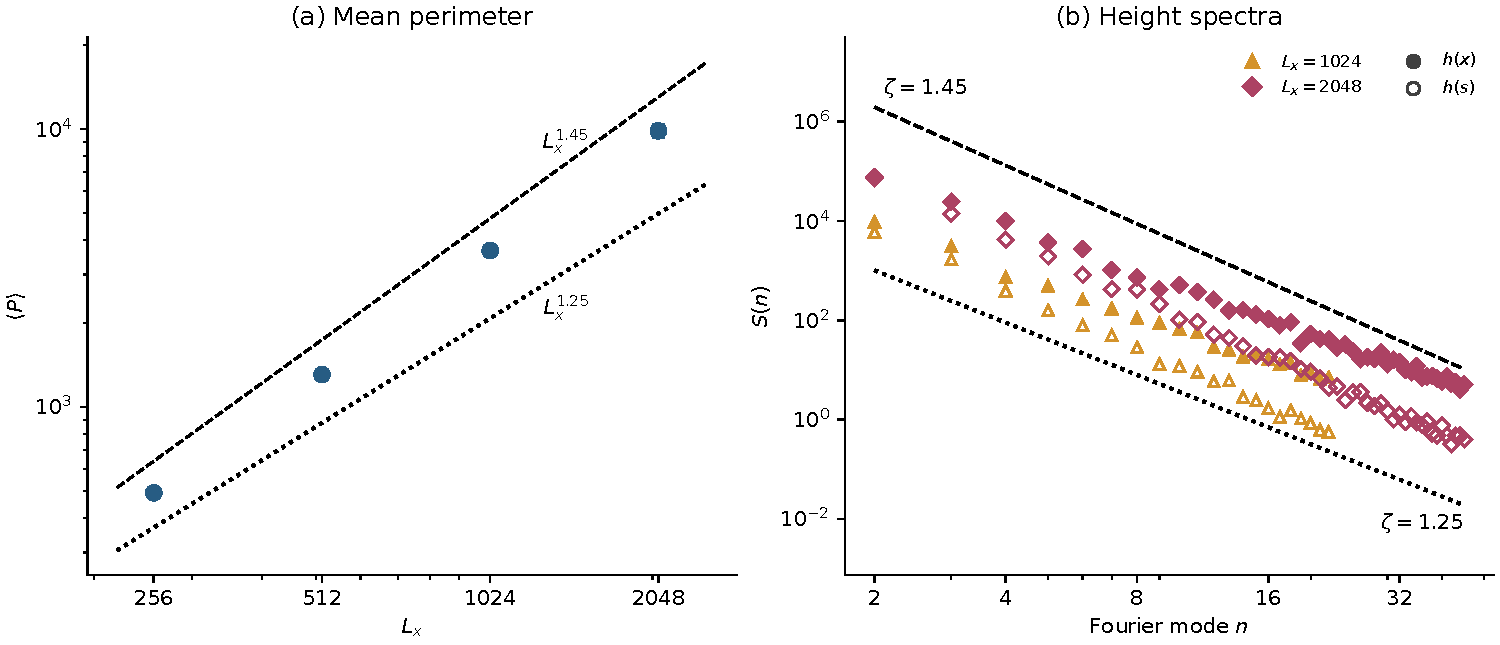
\includegraphics[width=\linewidth]{fig6_screw_scaling.pdf}
 \caption{Flat screw interfaces with anisotropic disorder ($a=1$),
 $\hat{\boldsymbol b}$ parallel to the mean interface direction,
 and $L_y=2L_x$.
 (a) Mean perimeter versus $L_x$.
 Error bars give $95\%$ bootstrap intervals for the mean.
 The black dashed and dotted lines have slopes $1.45$ and $1.25$,
 respectively.
 (b) Spectra $S(n)=\langle|\widehat h_n|^2\rangle$ versus the mode
 index $n$ for $L_x=1024$ and $2048$, with $2\leq n\leq45L_x/2048$.
 Filled symbols represent $h_x(x)$ and open symbols represent $h_s(s)$.
 The black dashed and dotted lines have slopes $-3.9$ ($\zeta=1.45$)
 and $-3.5$ ($\zeta=1.25$), with freely chosen amplitudes.
 Each contour has equal weight in the disorder average.}
 \label{fig:screw-scaling}
\end{figure}

\subsubsection{\texorpdfstring{$45^\circ$}{45 degrees}}
\label{sec:flat-45}

For the $45^\circ$ orientation, $\hat{\boldsymbol b}$ makes an angle of
$45^\circ$ with the mean interface direction. We use the same system
sizes, aspect ratio and numbers of realizations as above.
Figure~\ref{fig:diagonal-profiles} shows a depinning configuration with
long segments and a large-scale tilt.
At $L_x=2048$, about $57\%$ of the contour length has its tangent within
$30^\circ$ of the direction perpendicular to $\hat{\boldsymbol b}$,
and about $3\%$ within $30^\circ$ of $\hat{\boldsymbol b}$.

\begin{figure}[H]
 \centering
 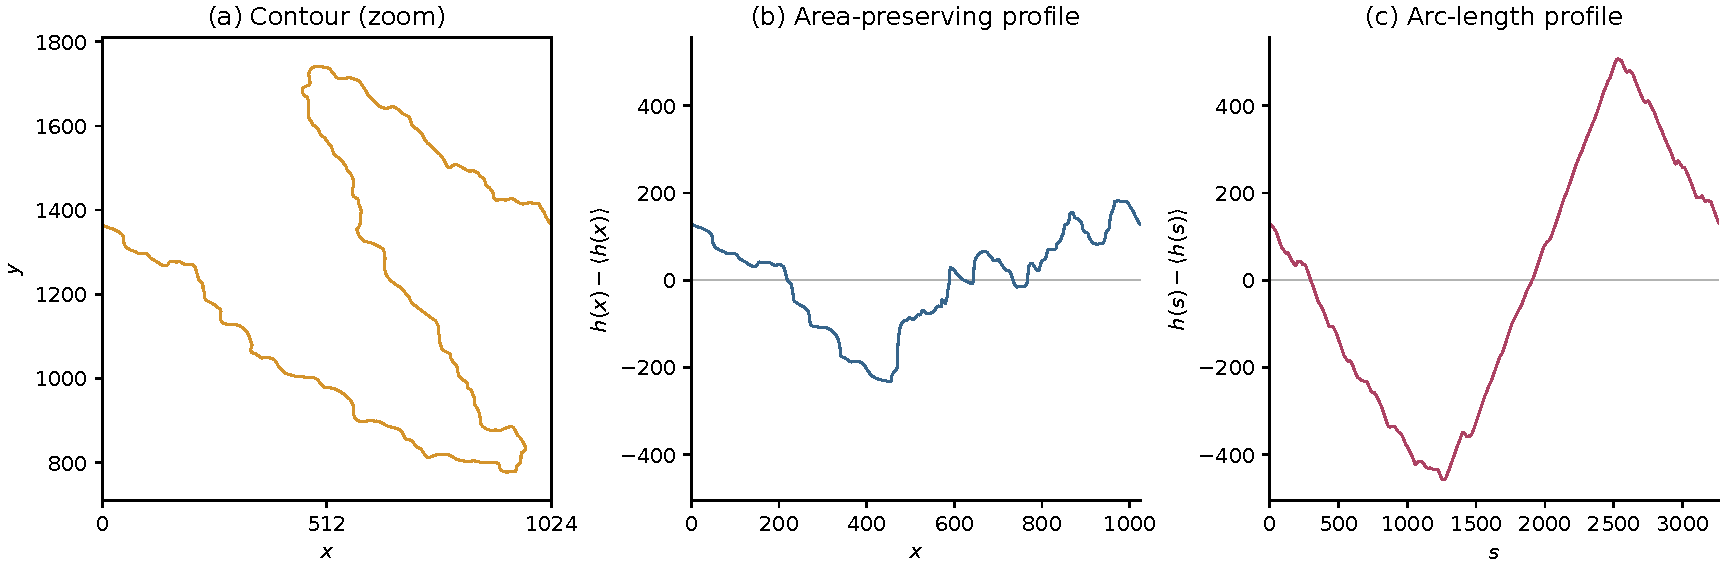
\includegraphics[width=\linewidth]{fig15_diagonal_profiles.pdf}
 \caption{Flat $45^\circ$ interface with anisotropic disorder ($a=1$) at
 $L_x=1024$, with perimeter $P=3262.98$.
 (a) Enlarged view of the full depinning contour.
 (b) Area-preserving profile $h(x)$.
 (c) Height $h(s)=y(s)$ along the contour, parametrized by arc length
 $s\in[0,P)$.
 In (b,c), the means $\langle h(x)\rangle$ and
 $\langle h(s)\rangle$ are subtracted, respectively.}
 \label{fig:diagonal-profiles}
\end{figure}

The mean perimeter grows approximately as
$\mathbb E[P]\propto L_x^{1.44}$, as shown in
Fig.~\ref{fig:diagonal-scaling}(a), close to the screw case.
The ratio $\mathbb E[P]/L_x$ increases from $1.43$ at $L_x=256$
to $3.56$ at $L_x=2048$.
Figure~\ref{fig:diagonal-scaling}(b) shows $S(n)$, as for the screw
orientation.
At $L_x=2048$, $h_s$ gives $\zeta\simeq1.26$ for $2\leq n\leq11$ and
$0.98$ at larger $n$, while $h_x$ gives $\zeta\simeq0.52$ over all the
modes shown.
At $L_x=2048$ and $q\leq0.03$, the effective exponents are
$\zeta_x\simeq0.55$ and $\zeta_s\simeq1.10$.
The two height representations differ strongly, since $32\%$ and
$46\%$ of the columns cross the contour more than once at $L_x=1024$
and $2048$, respectively.
As for the screw orientation, these slopes do not establish a
universality class.

\begin{figure}[H]
 \centering
 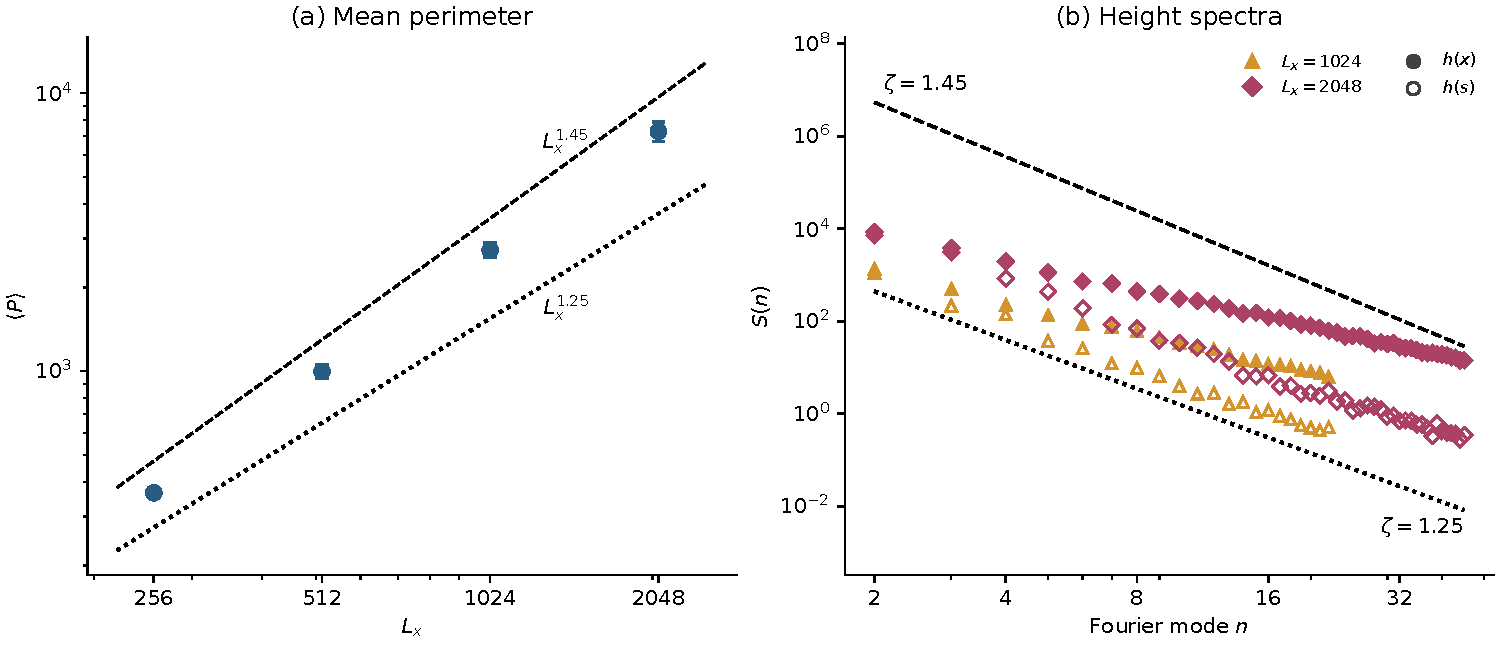
\includegraphics[width=\linewidth]{fig16_diagonal_scaling.pdf}
 \caption{Flat $45^\circ$ interfaces with anisotropic disorder ($a=1$),
 $\hat{\boldsymbol b}$ at $45^\circ$ from the mean interface direction,
 and $L_y=2L_x$.
 (a) Mean perimeter versus $L_x$.
 Error bars give $95\%$ bootstrap intervals for the mean.
 The black dashed and dotted lines have slopes $1.45$ and $1.25$,
 respectively.
 (b) Spectra $S(n)=\langle|\widehat h_n|^2\rangle$ versus the mode
 index $n$ for $L_x=1024$ and $2048$, with $2\leq n\leq45L_x/2048$.
 Filled symbols represent $h_x(x)$ and open symbols represent $h_s(s)$.
 The black dashed and dotted lines have slopes $-3.9$ ($\zeta=1.45$)
 and $-3.5$ ($\zeta=1.25$), with freely chosen amplitudes.
 Each contour has equal weight in the disorder average.}
 \label{fig:diagonal-scaling}
\end{figure}
